\subsection{Ergebnisse und Auswertung} \label{sec:ErgebnisseAAS}
  
  In Tabelle \ref{tab:ErgebnisseAAS} befinden sich die Ergebnisse der Standardaddition. In Abbildung \ref{fig:KalibriergeradeBlei} ist die entsprechende Kalibriergerade dargestellt. Folgende Parameter der Kalibriergeraden wurden bestimmt: Steigung $b = \SI[mode=text,separate-uncertainty]{0.00107(8)}{AU\per ppm}$, Ordinatenabschnitt $a = \SI[mode=text, separate-uncertainty]{0.0269(9)}{AU}$, Bestimmtheitsmaß $R^2 = 0.9396$, Reststandardabweichung $s_y = 0.002067$, F-Wert $F = 202.1434$ und Freiheitsgrade $df = 13$. Die Konzentration der Probe, $c_{Probe}$ wird über den Schnittpunkt der Kalibriergeraden mit der $x$-Achse bestimmt:
  
    \begin{equation}
      c_{Mess.} = |\frac{a}{b}|.
    \end{equation}
  Daraus berechnet sich die Probenkonzentration in den Kalibrierstandards zu \SI[mode=text]{25.1}{ppm}. Die tatsächliche Konzentration der Probe berechnet sich gemäß der Verdünnungsregel zu
  
    \begin{equation}
      c_{Probe} = \frac{c_{Mess.} V_{Mess.}}{V_{Probe}} = 5 c_{Mess.} = \SI[mode=text]{125.7}{ppm}.
    \end{equation}
  Der Vertrauensbereich für $\alpha = 0.05$ ($N = 15, t = 2.16$) kann über die Standardabweichung der Kalibriergeraden berechnet werden:
  
    \begin{equation}
      \begin{split}
        s_x &= \frac{s_y}{b} \sqrt{\frac{1}{N} + \frac{\overline{y}^2}{b^2 \sum_{i=1}^N \left(x_i - \overline{x}\right)^2}} \\
            &= \frac{0.002067}{0.00107} \sqrt{\frac{1}{15} + \frac{0.0376^2}{0.00107^2 \cdot 750}} = \SI[mode=text]{2.53}{ppm} \\
   \Rightarrow s_c &= \frac{V_{Mess.}}{V_{Probe}} s_x = 5 s_x = \SI[mode=text]{12.6}{ppm} \\
   \Rightarrow T_c &= s_c t = \SI[mode=text]{27.3}{ppm}.
      \end{split}
    \end{equation}
  Damit ist das Ergebnis: $c_{Probe} = \SI[mode=text, multi-part-units = brackets, separate-uncertainty]{126(27)}{ppm} \left(N = 15, s_c = \pm \SI[mode=text]{12.6}{ppm}, \alpha = 0.05\right)$.
  
  \begin{figure}[H]
    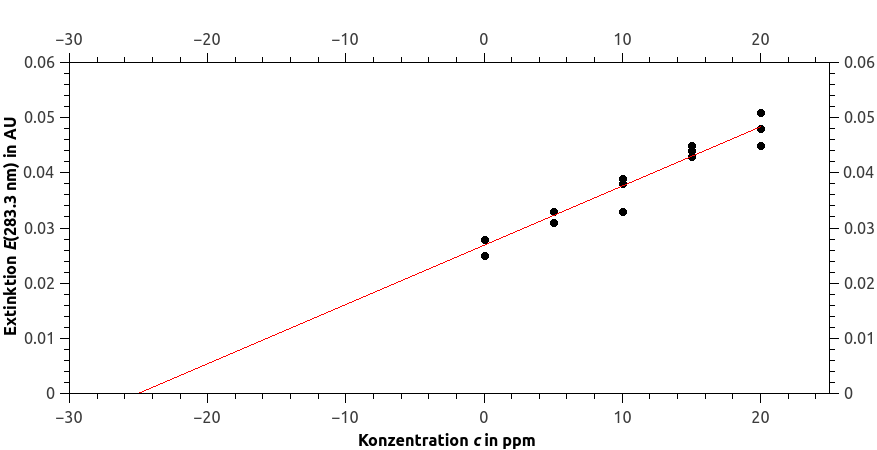
\includegraphics[scale=0.5, center]{images/KalibriergeradeAASPb.png} 
    \caption[Messdaten und Kalibriergerade für die AAS von \ch{Pb}, Quelle: Autor]{Messdaten und Kalibriergerade für die AAS von \ch{Pb} in der Form $y = a + bx$.}
    \label{fig:KalibriergeradeBlei}
  \end{figure}
  
  \begin{table}[H]
    \centering
    \caption[Ergebnisse AAS, Quelle: Autor]{Ergebnisse der AAS-Bestimmung von Blei}
    
    \label{tab:ErgebnisseAAS}   
    \begin{tabular}{@{}l|lllll|lp{4.5cm}l@{}}
      \toprule
      Standard & aliquoter Teil & $c_{Std.}$ in \si{ppm} & $V_{Std.}$ in \si{\milli\liter} & $V_{Ges.}$ in \si{\milli\liter} & $V_{Probe}$ in \si{\liter} & $E\left(\SI[mode=text]{283.3}{\nano\meter}\right)$ in AU \\ \midrule
        I & 1/10 & 0.0 & 0.0 & 50.0 & 10.0 & 0.028 \\
        I & 1/10 & 0.0 & 0.0 & 50.0 & 10.0 & 0.028 \\
        I & 1/10 & 0.0 & 0.0 & 50.0 & 10.0 & 0.025 \\
       II & 1/10 & 5.0 & 5.0 & 50.0 & 10.0 & 0.033 \\
       II & 1/10 & 5.0 & 5.0 & 50.0 & 10.0 & 0.031 \\
       II & 1/10 & 5.0 & 5.0 & 50.0 & 10.0 & 0.033 \\
     III  & 1/10 & 10.0 & 10.0 & 50.0 & 10.0 & 0.033 \\
     III  & 1/10 & 10.0 & 10.0 & 50.0 & 10.0 & 0.038 \\
     III  & 1/10 & 10.0 & 10.0 & 50.0 & 10.0 & 0.039 \\
       IV & 1/10 & 15.0 & 15.0 & 50.0 & 10.0 & 0.044 \\
       IV & 1/10 & 15.0 & 15.0 & 50.0 & 10.0 & 0.043 \\
       IV & 1/10 & 15.0 & 15.0 & 50.0 & 10.0 & 0.045 \\
        V & 1/10 & 20.0 & 20.0 & 50.0 & 10.0 & 0.045 \\
        V & 1/10 & 20.0 & 20.0 & 50.0 & 10.0 & 0.051 \\
        V & 1/10 & 20.0 & 20.0 & 50.0 & 10.0 & 0.048 \\ \bottomrule
    \end{tabular}
  \end{table}
